% Chapter 5

\chapter{Time Series} % Main chapter title

\label{Chapter5} % For referencing the chapter elsewhere, use \ref{Chapter5} 

\lhead{Chapter 5. \emph{Time Series}} % This is for the header on each page - perhaps a shortened title

%----------------------------------------------------------------------------------------

This chapter will use time series analysis to generate models to make forecasts for futures prices in various national stock market indices. Firstly three base systems will be considered, these are simple concepts and will be used as a bench mark against which the following time series models will be compared, and if they can't produce superior results won't be considered further. the base systems are the naive method which simply uses the previous value for the forecast of the next value, the average method in which the forecast is simply the mean of the pervious values and the drift method. The drift method is the average change encountered in the historical data and is equivalent to drawing a striaght line between the first and last observation. Subsequent time series models are developed using exponential smoothing methods, ARIMA techniques and finally hybrid methods.

\section{Base results}
Three base systems - mean, naive and drift were used to generate results as a starting point from which subsequent time series models can be compared. 

Figure \ref{fig:chp5_ts_dax} shows the three methods being applied to a data set derived from the German Dax. The models were trained on the first 3000 observations and tested on the remaining 528. The results of applying these simple models against the test data can be seen in Table \ref{tab:chp_ts:sma}.

%label - tab:chp_ts:sma
% latex table generated in R 3.1.0 by xtable 1.7-3 package
% Tue May 27 13:22:33 2014
\begin{table}[ht]
\centering
\caption[Simple forecasting methods.]{Mean, Naive and Drift methods applied to 
         to the Dax.} 
\label{tab:chp_ts:sma}
\begin{tabular}{llcccc}
  \toprule  & RMSE & MAE & MPE & MAPE & MASE \\ 
  \midrule Mean Training Set & 1394 & 1183 & -8 & 25 & 1 \\ 
  Mean Test Set & 208 & 163 & 2 & 3 & 3 \\ 
  Naive Training Set & 84 & 61 & -0 & 1 & 0 \\ 
  Naive Test Set & 303 & 263 & -5 & 5 & 4 \\ 
  Drift Training Set & 84 & 61 & -0 & 1 & 0 \\ 
  Drift Test Set & 302 & 262 & -5 & 5 & 4 \\ 
   \bottomrule \end{tabular}
\end{table}


Figure \ref{fig:chp5_ts_dax} is a plot of the forecast from these models generated against the training set and forecasting the closing price at the end of the test period. The Naive and Drift algorithms forecast similar values while the Mean method produces a markedly lower value.

\begin{figure}[tbh]
\centering
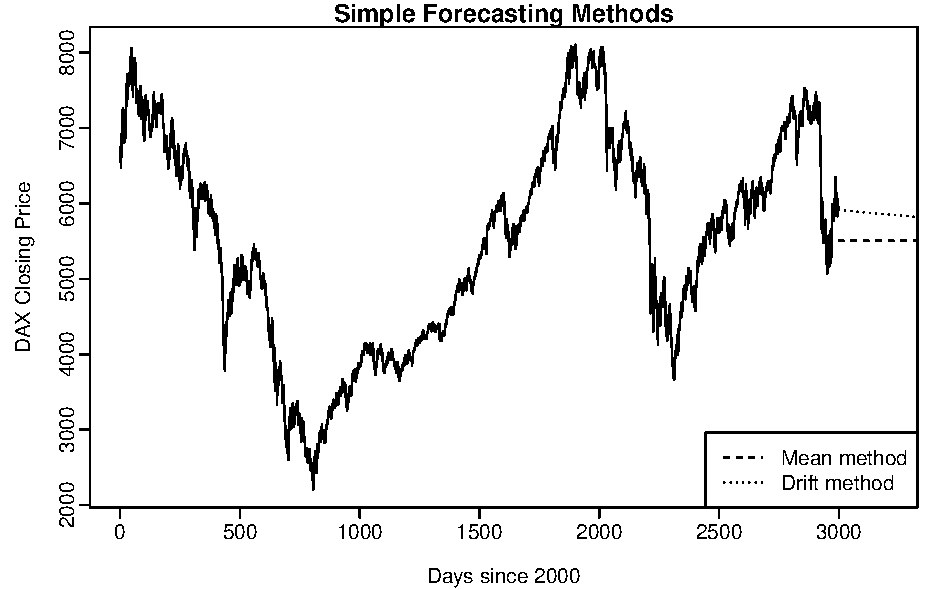
\includegraphics{Figures/chp_ts_dax1}
\caption[Results of simple modelling methods.]{Results of simple modelling methods.}
\label{fig:chp5_ts_dax}
\end{figure}

Figure \ref{fig:chp_ts_dax_act} is the same as Figure \ref{fig:chp5_ts_dax} except the actual data encountered during the foecast period has been added.

\begin{figure}[tbh]
\centering
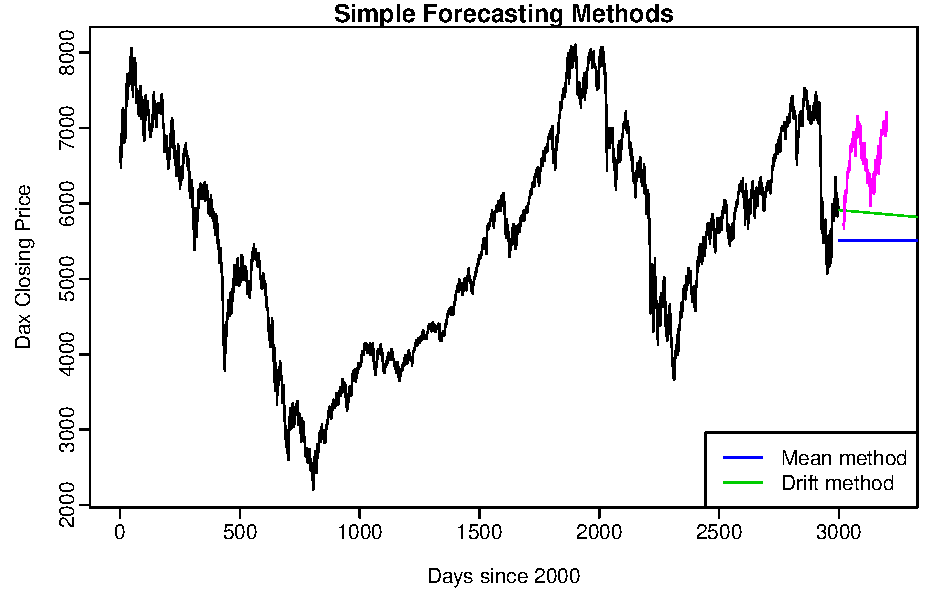
\includegraphics{Figures/chp_ts_dax1_plus_act_data}
\caption[Results of simple modelling methods and actual data.]{Results of simple modelling methods with actual data in forecast period added.}
\label{fig:chp_ts_dax_act}
\end{figure}

\section{Exponential Smoothing}

Using Rob J Hyndman's forecast package and the ets() function, a variety of exponential smoothing methods can be applied to sample data \citep{Hyndman08automatictime}. Table \ref{tab:tax_em} lists fifteen possibilities when one combines trend and seasonality. In fact Hyndman extends this further by allowing the error term to be either added or multiplied against the results. 

\begin{table}[ht]
\centering
\caption[Taxonomy of exponential smoothing methods.]{of exponential smoothing methods.} 
\label{tab:tax_em}
\begin{tabular}{lccc}
  \toprule 
            & \multicolumn{3}{c}{Seasonal Component} \\
  \cmidrule(r){2-4}
  Trend     & N      & A          & M       \\ 
  Component &(None)  &(Additive)  & (Multiplicative)  \\
  \midrule 
  N (None) & (N,N)&(N,A)&(N,M)  \\ 
  A (Additive) & (A,N)&	(A,A)&(A,M)  \\ 
  Ad (Additive damped) &(Ad,N)&(Ad,A)&(Ad,M) \\ 
  M (Multiplicative) &(M,N)&(M,A)&(M,M)  \\ 
  Md (Multiplicative damped) &(Md,N)&(Md,A)&(Md,M) \\ 
   \bottomrule \end{tabular}
\end{table}

Note - Hymndman: hard to beat the ets model, 37 mins.


% ------ NEW PAGE --------------------------
\newpage
\section{ARIMA Models}
\label{arima_models}

The process of fitting an ARIMA model to a time series involves the following general steps:

\begin{enumerate}
\item Plot the data to get a general feel for the time series and to establish if it is stationary.
\item Stabilize any variance in the data with a transformation process such as the Box-Cox method.
\item Arima models work with stationary data, so if necessary, take differences of the data until it is stationary.
\item Examine the auto-correlation and partial auto-correlation (ACF/PACF) plots in order to determine if an AR(p) or MA(q) model is appropriate.
\item Test the chosen model(s), using the AICc to determine if a better model is available.
\item Check the residuals from the best model by plotting the ACF, and doing a portmanteau test on them. If the results from these tests do not look like white noise, a modified model may be required.
\item Finally, once the residuals have a similar pattern to white noise, the model can be used to generate forecasts.
\end{enumerate}


In recent years automatic forecasting algorithms have become available and widely used \citep{Hyndman08automatictime}. These are necessary in a variety of circumstances, especially when organisations are faced with the need to repeatedly carry out a large number of forecasts and the human effort required renders manual means impractical. The auto.arima() function found in R's \textquotedblleft forecast" package is an example of an automatic algorithm for arima models. This function automates steps 3, 4, and 5 of those outlined previously in the general steps required for arima modelling. In the following sections, the general steps are followed in order to generate an arima model manually then the automatic algorithm is used for comparison purposes.

\subsection{Data Exploration}

The first step, as always is to explore the data. Figure \ref{fig:chp_ts_ftse_2000_13} shows the UK's FTSE 100 index between the years 2000 to 2013. Over this time period the series has shown strong trends to move up and down and a uniform variance. Because the time series is non-stationary it will need to be transformed into a stationary series before arima modelling can be undertaken.

\begin{figure}[tbh]
\centering
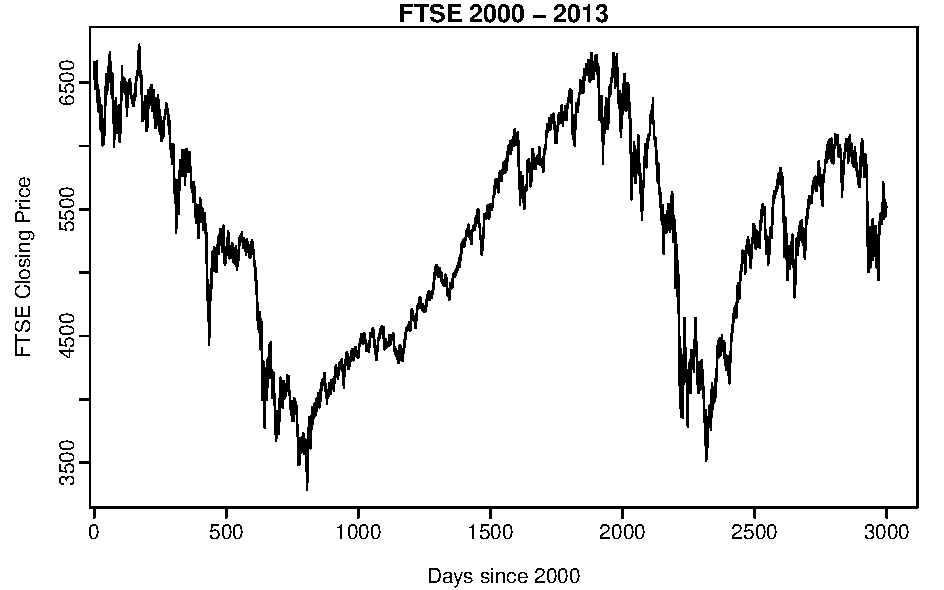
\includegraphics{Figures/chp_ts_ftse_2000-13}
\caption[FTSE 2000-13.]{UK's FTSE 100 index between the years 2000 to 2013.}
\label{fig:chp_ts_ftse_2000_13}
\end{figure}

\subsection{Adjusting for non-uniform variance and non-stationariness}
The variance within the FTSE time series is relatively uniform and thus this data set doesn't need stabilizing with regard to this. If it did a Box-Cox transformation could be used. However, the FTSE 100 over this time period exhibits marked non-stationariness and requires adjusting accordingly. Differencing is a technique to make a data set stationary. Instead of using the actual observations the differences between two adjacent points are used and this is known as the first difference. If the data set still isn't stationary the difference between consecutive points in the differenced data set can used, this is the difference of the differences and is known as the second difference. Figure \ref{fig:chp_ts_ftse_2000_13_diff} shows the FTSE data set after the first differences have been taken.  The resulting data set is now stationary.

\begin{figure}[tbh]
\centering
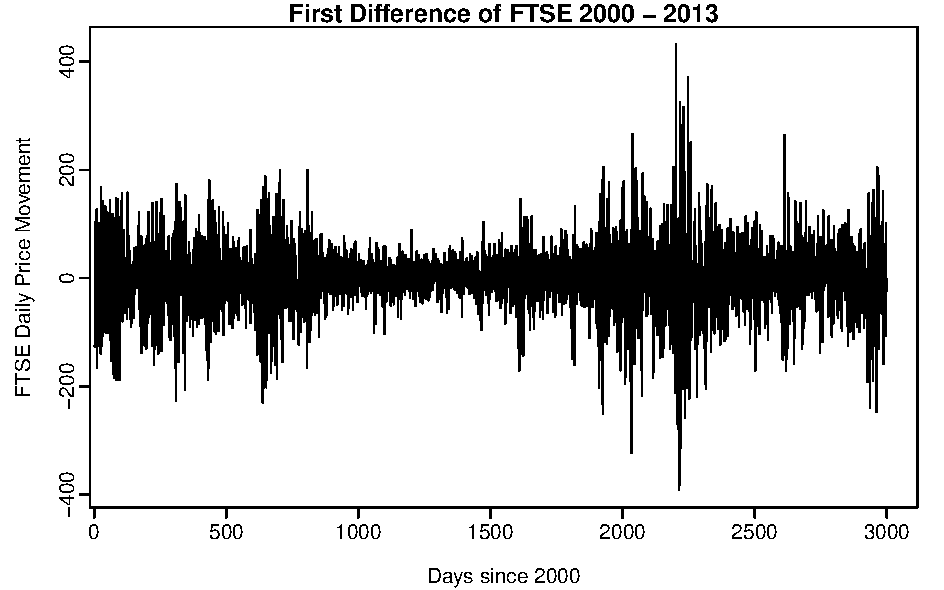
\includegraphics{Figures/chp_ts_ftse_2000-13_diff}
\caption[FTSE 2000-13 Diff.]{FTSE 2000-13 Diff.}
\label{fig:chp_ts_ftse_2000_13_diff}
\end{figure}

\subsection{Examine ACF / PACF}
With a stationary data set, the next stage is to investigate the auto-correlation and partial auto-correlation (ACF/PACF) plots in order to help in the model selection process (see section \ref{sec:acf} for details of ACF and PACF). The ACF and PACF for the FTSE data set can be seen in Figures \ref{fig:chp_ts_ftse_2000-13_diff_acf} and \ref{fig:chp_ts_ftse_2000-13_diff_pacf}. 

If ultimately the arima model is of the form ARIMA(p,d,0) or ARIMA(0,d,q) then the ACF and PACF plots are useful in helping to define values for p or q. In the event that both p and q are positive, the ACF and PACF are not helpful in deducing the values for p and q. An ARIMA(p,d,0) model may be appropriate if the ACF and PACF plots of the stationary data exhibit an exponentially decaying pattern in the ACF and a large spike at lag p in PACF plot. Conversely an ARIMA(0,d,q) model may be appropriate if the PACF is decaying exponentially and there is there is a significant spike in the ACF plot at lag q. Considering the ACF and PACF plots in Figures \ref{fig:chp_ts_ftse_2000-13_diff_acf} and \ref{fig:chp_ts_ftse_2000-13_diff_pacf}, neither of the two patterns are observed and thus an arima model where both p and q are positive is likely.

\begin{figure}[tbh]
\centering
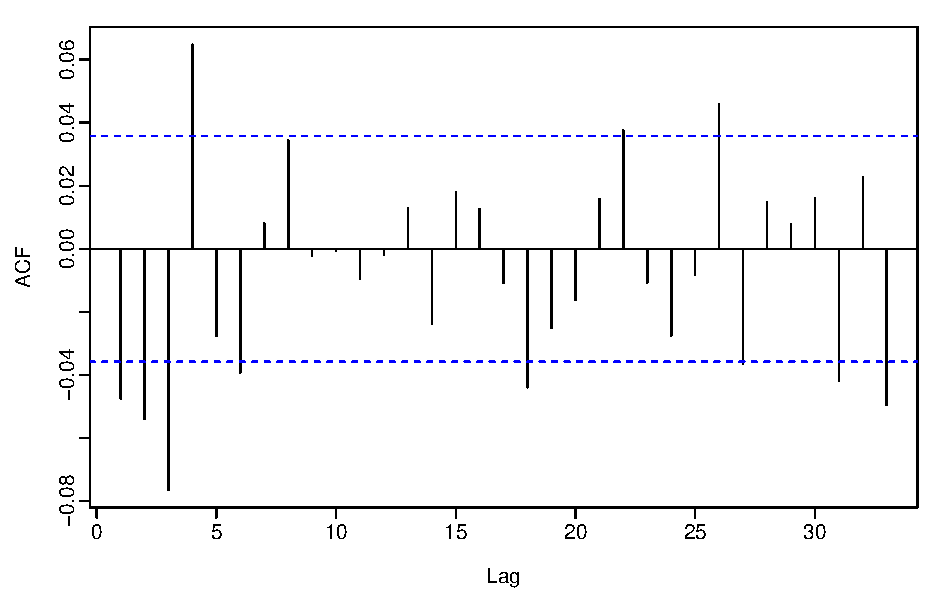
\includegraphics{Figures/chp_ts_ftse_2000-13_diff_acf}
\caption[FTSE 2000-13 Diff.]{ACF of Diff FTSE 2000-13.}
\label{fig:chp_ts_ftse_2000-13_diff_acf}
\end{figure}

\begin{figure}[tbh]
\centering
\includegraphics{Figures/chp_ts_ftse_2000-13_diff_pacf}
\caption[FTSE 2000-13 Diff.]{PACF of Diff FTSE 2000-13.}
\label{fig:chp_ts_ftse_2000-13_diff_pacf}
\end{figure}

%\begin{figure}[tbh]
%\centering
%%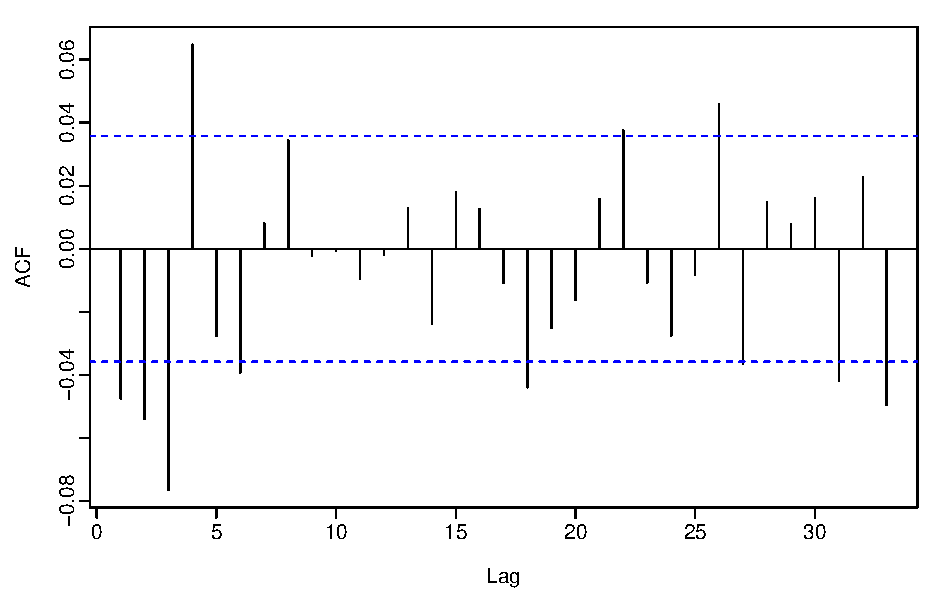
\includegraphics[width=15cm]{Figures/chp_ts_ftse_2000-13_diff_acf}
%\includegraphics[width=14cm, height=12cm]{Figures/chp_ts_ftse_2000-13_diff_acf_tsd}
%\caption[FTSE 2000-13 ACF / PACF.]{Difference, ACF and PACF plots for the FTSE 2000-13.}
%\label{fig:chp_ts_ftse_2000_13_diff_acf_tsd}
%\end{figure}

\subsection{Try the chosen model(s)}
The next step is to try the chosen model along with a few viable alternatives. 

%Akaike’s Information Criterion (AIC) and Bayesian Information Criterion (BIC) are useful for determining the optimum order of an ARIMA model, and are typically used as a measure of how well the model fits the data. 
%\[ AIC = -2 log (L) + 2 (p+q+k+1) \]
%where:\\
%$ L $ is the likelihood of the data\\ 
%$ k = 1$ if $c != 0 $ and $ k=0$ if $c != 0$\\
%Note that the last term in parentheses is the number of parameters in the model, the variance of the residuals.
%
%For ARIMA models, the corrected AIC can be written as:
%\[ AIC_{c} = AIC + \dfrac{2 (p+q+k+1)(p+q+k+2)}{T-p-q-k-2} \]
%
%The Bayesian Information Criterion can be expressed as:
%\[ BIC = AIC + log(T)(p+q+k+1) \]
%
%Table \ref{tab:chp_ts:arima_res_r} shows the AIC, AICc and BIC accuracy measures for a selection of arima models applied to the FTSE data set. On all three measures the arima(2,1,3) model has the lowest value.

%label - tab:chp_ts:arima_res_r
% latex table generated in R 3.1.0 by xtable 1.7-3 package
% Thu Aug 21 07:23:05 2014
\begin{table}[ht]
\centering
\caption[AIC, AICc and BIC results from alternative ARIMA models]{AIC, AICc and BIC results from alternative ARIMA models.} 
\label{tab:chp_ts:arima_res_r}
\begin{tabular}{lccc}
  \toprule Model & AIC & AICc & BIC \\ 
  \midrule ARIMA(3,1,1) & 33598.5 & 33598.5 & 33628.5 \\ 
  ARIMA(3,1,2) & 33594.6 & 33594.6 & 33630.6 \\ 
  ARIMA(3,1,3) & 33596.1 & 33596.1 & 33638.1 \\ 
  ARIMA(2,1,1) & 33616.4 & 33616.4 & 33640.4 \\ 
  ARIMA(2,1,2) & 33618.1 & 33618.1 & 33648.1 \\ 
  ARIMA(2,1,3) & 33594.1 & 33594.1 & 33630.1 \\ 
   \bottomrule \end{tabular}
\end{table}


\subsection{Model Residuals}
A so-called residual is the difference between an observation and its forecast. In forecasting a time series, residuals are calculated from a one-step forecast.  A one-step forecast is based on all observations from the start of the series until the previous observation to which the forecast applies to. Thus the number of data points used to calculate the one-step forecast increases as the forecast proceeds through the time series.  An alternative is cross-sectional forecasting which uses all the points in the data set except the observation being predicted.

Knowledge of the residuals from the application of a model is important in establishing the validity of the model. There are two essential and two valuable properties that can be established by inspecting the model residuals. A good method of forecasting will produce a model in which the residuals are uncorrelated and have a zero mean. If a forecasting method doesn't comply with these two properties it can be improved upon. Correlation in residuals means that information is present in them that the model has missed and a non-mean is evidence of bias in the forecast. Adjusting for bias is straight forward, the mean value observed in the residuals can simply be added to all forecasts. Looking at Figure \ref{fig:chp_ts_ftse_2000_13_mean_residuals} it can be seen that the mean of the residuals is close to zero and this model doesn't have any bias.

\begin{figure}[!tbh]
\centering
\includegraphics{Figures/chp_ts_ftse_2000-13_mean_residuals}
\caption[FTSE 2000-13 residuals.]{The residuals from applying the arima model to the FTSE data set.}
\label{fig:chp_ts_ftse_2000_13_mean_residuals}
\end{figure}

Figure \ref{fig:chp_ts_ftse_2000_13_acf_residuals} is the plot of the residuals of the arima model applied to the FTSE data set. WHAT DOES IT SHOW \label{(todo-acf)}

\begin{figure}[!tbh]
\centering
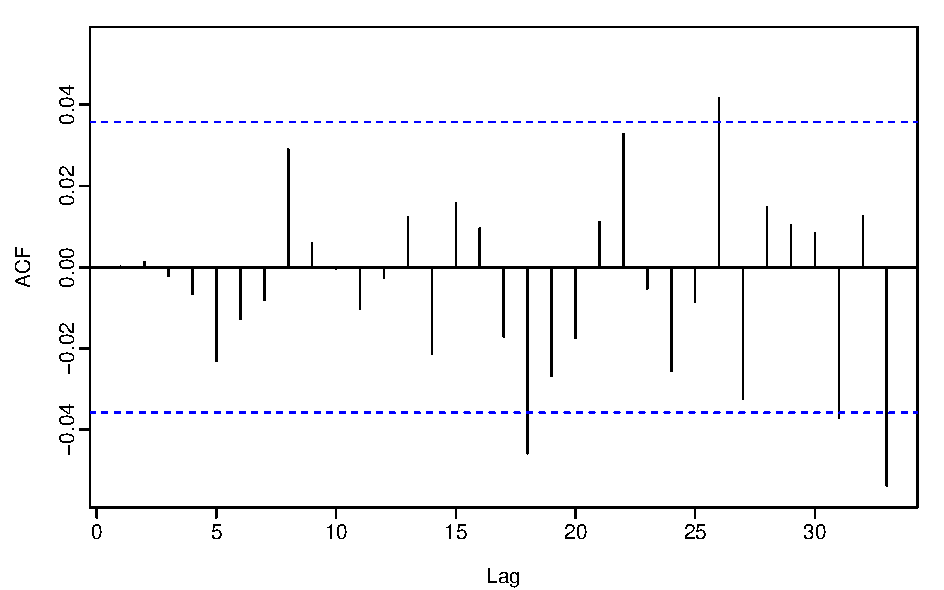
\includegraphics{Figures/chp_ts_ftse_2000-13_acf_residuals}
\caption[FTSE 2000-13 ACF of residuals.]{ACF plot of the residuals from applying the arima model to the FTSE data set.}
\label{fig:chp_ts_ftse_2000_13_acf_residuals}
\end{figure}

Two additional properties of the residuals that are desirable, though not necessary, are constant variance and normal distribution. If these two conditions are met, the calculation of the prediction interval inthe forecast step is easier. From Figure \ref{fig:chp_ts_ftse_2000_13_mean_residuals} it can be seen that the residuals have relatively constant variance and from Figure \ref{fig:chp_ts_ftse_2000_13_hist_residuals} it can be seen that they are normally distributed.

\begin{figure}[!tbh]
\centering
\includegraphics{Figures/chp_ts_ftse_2000-13_hist_residuals}
\caption[FTSE 2000-13 - Histogram of residuals.]{Histogram of the residuals from applying the arima model to the FTSE data set.}
\label{fig:chp_ts_ftse_2000_13_hist_residuals}
\end{figure}

% Box Ljung test
Consideration of the ACF plots provides evidence for auto-correlation. However a more formal approach is to consider auto-correlation values together as a group as opposed to individually. The Box-Ljung portmanteau test is just one such approach and Table \ref{tab:chp_ts:arima_res_rbox_l} lists the results of the Box-Ljung portmanteau test being applied to the residuals of the arima model. A large p-value is indicative of white noise and is the desirable situation for a good arima model.

%label - tab:chp_ts:arima_res_rbox_l
% latex table generated in R 3.1.0 by xtable 1.7-3 package
% Mon Jul 07 19:17:49 2014
\begin{table}[ht]
\centering
\caption[Box Ljung test of FTSE 100 ARIMA model residuals]{Box Ljung test of FTSE 100 ARIMA model residuals.} 
\label{tab:chp_ts:arima_res_rbox_l}
\begin{tabular}{llcc}
  \toprule  & p-value & x-squared & df \\ 
  \midrule ARIMA(2,1,3)                    & 0.2328 & 20 & 24 \\ 
   \bottomrule \end{tabular}
\end{table}


\subsection{Calculate forecast}
Finally, after developing a model that meets the previous criteria a forecast can be generated. Table \ref{tab:chp_ts:ftse_100_fcast} shows the one-step forecast produced when the arima(3,1,2) model developed in the previous section is applied to the FTSE data set.
 
%label - tab:chp_ts:ftse_100_fcast
% latex table generated in R 3.1.0 by xtable 1.7-3 package
% Tue Aug 26 19:01:45 2014
\begin{table}[ht]
\centering
\caption[Forecast for FTSE 100 generated from the ARIMA model]{One-step ahead forecast for FTSE 100 generated from ARIMA(2,1,3) model.} 
\label{tab:chp_ts:ftse_100_fcast}
\begin{tabular}{lccccc}
  \toprule Date & Open & High & Low & Close & Forecast \\ 
  \midrule 20/12/2013 & 6585 & 6617 & 6577 & 6607 & 6560 \\ 
  23/12/2013 & 6607 & 6679 & 6606 & 6679 & 6598 \\ 
  24/12/2013 & 6679 & 6712 & 6672 & 6694 & 6666 \\ 
  27/12/2013 & 6694 & 6754 & 6694 & 6751 & 6692 \\ 
  30/12/2013 & 6751 & 6768 & 6718 & 6731 & 6743 \\ 
  31/12/2013 & 6731 & 6757 & 6731 & 6749 & 6730 \\ 
   \bottomrule \end{tabular}
\end{table}



\subsection{Automatic Arima Modelling}
As explained previously the automatic arima modelling algorithm in the R forecast package automates steps 3 to 5 in the general steps used in the modelling process as outlined in section \ref{arima_models}. The function uses a variation of the Hyndman and Khandakar algorithm which obtains an arima model by the minimisation of the AICc and combination with unit root tests. KPSS tests are used to establish the number of differences, d, required to get a stationary time series. The p and q values are then obtained by choosing the model that minimises the AICc for the differenced data. 


Table \ref{tab:chp_ts_arima_models} 
%label - tab:chp_ts_arima_models
% latex table generated in R 3.1.0 by xtable 1.7-3 package
% Sat Aug 23 08:35:18 2014
\begin{table}[ht]
\centering
\caption[ARIMA models chosen for the indice data sets]{ARIMA models chosen to forecast future values in the national indice data sets.} 
\label{tab:chp_ts_arima_models}
\begin{tabular}{lc}
  \toprule Market & ARIMA Model \\ 
  \midrule DAX & ARIMA(3,1,3)                    \\ 
  CAC & ARIMA(2,1,3)                    \\ 
  FTSE & ARIMA(2,1,3)                    \\ 
  Dow & ARIMA(1,1,2)                    \\ 
  Nikkei & ARIMA(2,1,3)                    \\ 
  AORD & ARIMA(1,1,0)                    \\ 
   \bottomrule \end{tabular}
\end{table}




\section{Trading Systems}
Having developed forecasts based on arima models these can be passed into a trading system.

Table \ref{tab:chp_ts:arima1} results from from ts1 code - Arima1 - ARIMA(3,1,3)
%label - tab:chp_ts:arima1
% latex table generated in R 3.1.0 by xtable 1.7-3 package
% Sun Jun 29 08:18:19 2014
\begin{table}[ht]
\centering
\caption[Forecasts generated by the ARIMA models used in the System 1 algorithm]{Forecasts generated by the ARIMA models used in the System 1 algorithm.} 
\label{tab:chp_ts:arima1}
\begin{tabular}{lcccccc}
  \toprule Mkt & LongPL & ShortPL & L Win \% & Av L PL & S Win \% & Av S PL \\ 
  \midrule Dax & -644 & -1881 & 50 & -3 & 41 & -7 \\ 
  CAC & 1555 & 850 & 59 & 6 & 51 & 3 \\ 
  FTSE & 531 & -708 & 53 & 2 & 46 & -2 \\ 
  Dow & 3130 & -1766 & 58 & 14 & 48 & -6 \\ 
  Nikkei & 41 & -1157 & 48 & 0 & 45 & -5 \\ 
  AORD & 679 & -204 & 55 & 3 & 49 & -1 \\ 
   \bottomrule \end{tabular}
\end{table}



Table \ref{tab:chp_ts:arima2} results from from ts1 code - Arima1 - ARIMA(3,1,3)
%label - tab:chp_ts:arima2
% latex table generated in R 3.1.0 by xtable 1.7-3 package
% Tue Aug 19 13:19:29 2014
\begin{table}[ht]
\centering
\caption[Results from trading System 2 using the forecasts generated by the ARIMA models]{Results from trading System 2 using the forecasts generated by the ARIMA models.} 
\label{tab:chp_ts:arima2}
\begin{tabular}{lcccccc}
  \toprule Mkt & LongPL & ShortPL & L Win \% & Av L PL & S Win \% & Av S PL \\ 
  \midrule DAX & 733 & -505 & 55 & 3 & 46 & -2 \\ 
  CAC & 545 & -80 & 53 & 2 & 47 & 0 \\ 
  FTSE & 941 & -383 & 54 & 3 & 46 & -2 \\ 
  Dow & 2598 & -2221 & 55 & 9 & 46 & -10 \\ 
  Nikkei & 179 & -916 & 50 & 1 & 47 & -4 \\ 
  AORD & 811 & -117 & 53 & 3 & 46 & 0 \\ 
   \bottomrule \end{tabular}
\end{table}

% ---------------------------------------------------------------
\section{Hybrid Arima Models}
Figure \ref{fig:chp_ts_rm_arima} shows the Rapid Miner process used to generate Arima models. The various components are as follows:

\begin{itemize}
\item Read CSV - reads in the appropriate data set.
\item Select Attribute (1) - selects the attribute that will be processed in the following steps.
\item Rename - renames the attribute selected in Select Attribute (1) to \textquotedblleft attr1" which is then used in the est of the steps. This component is used to make it easy to change the attribute without having to rename all the subsequent steps.
\item Moving Average - calculates a moving average of the time series (see section \ref{sec:chp2_sma} for details.) This provides the q in ARIMA(p,d,q) models.
\item Differentiate - calculates the difference in the time series and provides the d in ARIMA(p,d,q) models.
\item Lag - creates lag variables which are values of the attribute (the attribute itself, the moving average or the difference value) at earlier points in the time series.
\item Select Attribute (2) - selects the attributes that will be passed to the validation block. Attributes regaring today's values are removed because we are building a model to calculate them and don't want to \textquotedblleft peak" at them before the model is built.
\item Set Role - sets an attribute as the label to be predicted.

\end{itemize}

\begin{figure}[!tbh]
\centering
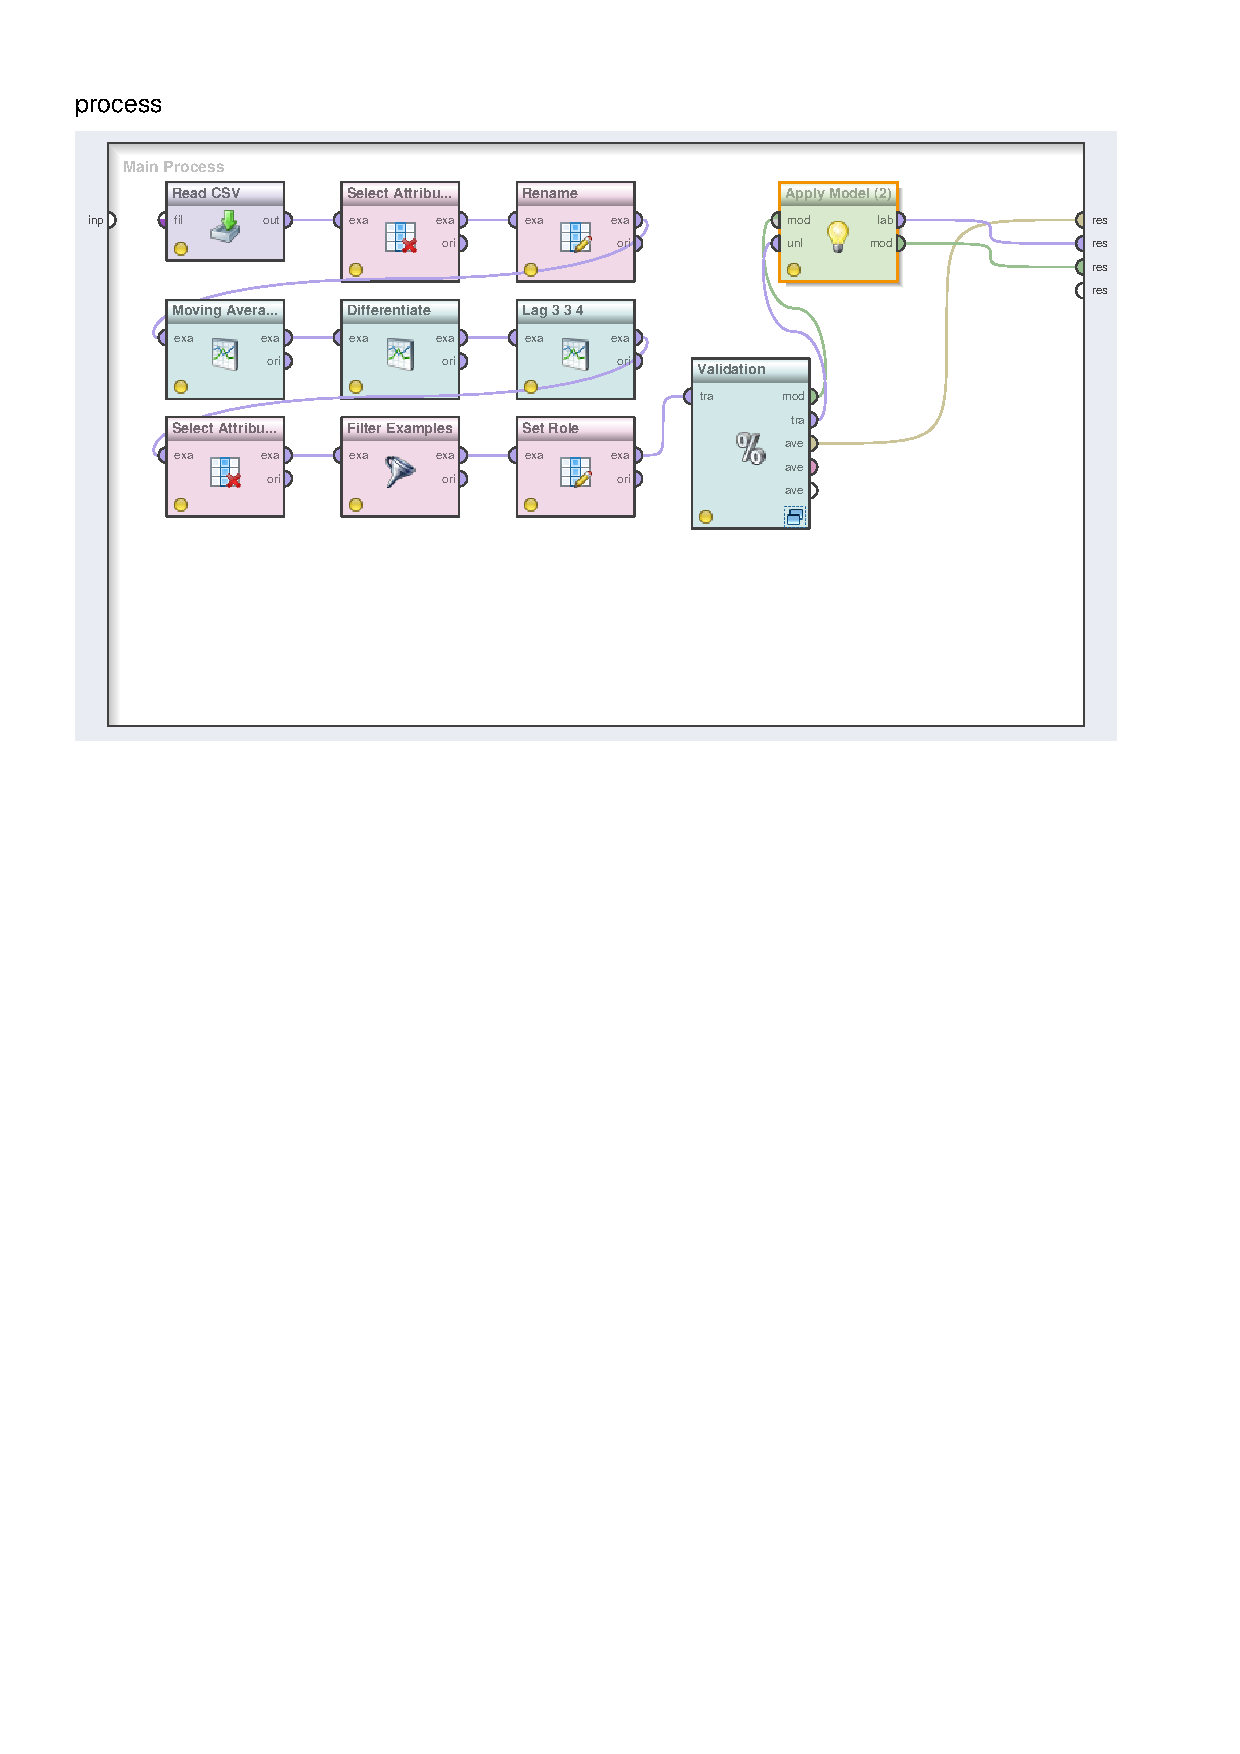
\includegraphics[width=12cm]{../Figures/chp_ts_rm_arima}
\caption[Rapid Miner Arima Process]{Rapid Miner Arima Process.}
\label{fig:chp_ts_rm_arima}
\end{figure}

Questions - should we pass the diff values to the model - just to flatten the series?

TO DO - auto forecast - on window - does model change? prediction any good? ets and arima ...

Table \ref{tab:chp_ts:arima_hybrid_reg} are the results of using the output of the arima-hybrid in a trading system.
%label - tab:chp_ts:arima_hybrid_reg
% latex table generated in R 3.1.0 by xtable 1.7-3 package
% Mon May 26 22:01:42 2014
\begin{table}[ht]
\centering
\caption[ts1 arima hybrid reg.]{ts1 arima hybrid reg.} 
\label{tab:chp_ts:arima_hybrid_reg}
\begin{tabular}{lcccccc}
  \toprule Mkt & LongPL & ShortPL & L Win \% & Av L PL & S Win \% & Av S PL \\ 
  \midrule Dax & 1964 & 1765 & 56 & 5 & 48 & 3 \\ 
   \bottomrule \end{tabular}
\end{table}


